\mode<presentation>
{
  %\usetheme{umbc4}
  %\setbeamercovered{dynamic}
}
\usepackage[english]{babel}
% or whatever

\usepackage[latin1]{inputenc}
% or whatever

\usepackage{times}
\usepackage[T1]{fontenc}
% Or whatever. Note that the encoding and the font should match. If T1
% does not look nice, try deleting the line with the fontenc.
%--------------------------------------------------------------------------------------------
%--- Other packages
\usepackage{pstricks}
\usepackage{pst-node}
\usepackage{pst-rel-points}
\usepackage{xspace}

%%%%%% Declarations Defined in custom-foils
%\setfootline{\insertshortauthor, \insertshortinstitute \hfill   \insertshorttitle \hfill \insertframenumber/\inserttotalframenumber} 
\newcommand{\mypart}[1]{%
  \frame[plain]{\mbox{}\vfill \psshadowbox{\huge #1} \vfill\mbox{}}
}
\author[karkare]{Amey Karkare \\ \url{karkare@cse.iitk.ac.in}}
\date[]{\scalebox{0.3}{\includegraphics{iitklogo.epsi}}}%
\institute[CSE, IITK]{\url{http://www.cse.iitk.ac.in/~karkare/cs738}\\Department of CSE, IIT Kanpur}
\title[CS738]{CS738: Advanced Compiler Optimizations}
\subtitle[]{}


\subtitle[]{\ \\{\LARGE Data Flow Analysis}\\}

\newcommand{\bbent}{{\it Entry}\xspace}
\newcommand{\bbext}{{\it Exit}\xspace}

\newcommand{\IN}{{\sf IN}\xspace}
\newcommand{\OUT}{{\sf OUT}\xspace}

\newcommand{\Pred}{{\sf PRED}\xspace}
\newcommand{\Succ}{{\sf SUCC}\xspace}

\newcommand{\Kill}{{\sf KILL}\xspace}
\newcommand{\Gen}{{\sf GEN}\xspace}

\newcommand{\cmt}[1]{{}}
\newcommand{\meet}{\ensuremath{\bigwedge}\xspace}
\newcommand{\join}{\ensuremath{\bigvee}\xspace}
\newcommand{\glb}{{\sf glb}\xspace}
\newcommand{\lub}{{\sf lub}\xspace}

%% Framed minipage %%%%%%%%%%%%%%%%%%%%%%%%%%%%%%%%%%%%
\newsavebox\TestBox
\newenvironment{frmminipage}[2][]
{\begin{lrbox}{\TestBox}\begin{minipage}[#1]{#2}}
{\end{minipage}\end{lrbox}\fbox{\usebox{\TestBox}}}


\newcommand{\mylabbox}[2]{{\small #1}\psframebox{#2}\phantom{\small #1}}

\newcommand{\tossa}{%
  \ensuremath{\stackrel{SSA\quad\ }{\scalebox{3}{$\Rightarrow$}}}}

\newcommand{\jstfy}{\mbox{\phantom{XX}}}

\newcommand{\dom}{\operatorname{dom}}
\newcommand{\sdom}{\operatorname{sdom}}
\newcommand{\idom}{\operatorname{idom}}

\newcommand{\DOM}{\operatorname{DOM}}
\newcommand{\DF}{\operatorname{DF}}

\begin{document}

\frame{\titlepage}
\frame{
  \frametitle{Agenda}
  \begin{itemize}[<+->]
  \item {\em Intraprocedural} Data Flow Analysis: Classical Examples
    \begin{itemize}
    \item Last lecture: Reaching Definitions
    \item Today: Available Expressions
    \item Discussion about the similarities/differences
    \end{itemize}
  \end{itemize}
}

\frame{
  \frametitle{Available Expressions Analysis}
  \begin{itemize}[<+->]
  \item An expression $e$ is available at a point $p$ if
    \begin{itemize}
    \item {\bf Every} path from the \bbent to $p$ has at least one evaluation of $e$
    \item There is no assignment to any component variable of $e$ {\bf after the last evaluation} of $e$ prior to $p$
    \end{itemize}
  \item Expression e is {\em generated} by its evaluation
  \item Expression e is {\em killed} by assignment to its component
    variables
  \end{itemize}
}

\frame{
  \frametitle{AvE Analysis of a Structured Program}
  \begin{center}
    \psset{unit=1mm}
    \begin{pspicture}(0,0)(50,30)
      %\psframe(0,0)(50,30)
      \putnode{s1}{origin}{25}{15}{%
        \psovalbox[fillstyle=solid,fillcolor=lightgray]{$d: x = y + z$}}
      \putnode{se}{s1}{0}{15}{}
      \putnode{sx}{s1}{0}{-15}{}
      \putnode{sl}{s1}{20}{0}{$s_1$}
      \ncline{->}{se}{s1}\Aput{$\IN(s_1)$}
      \ncline{->}{s1}{sx}\Aput{$\OUT(s_1)$}
    \end{pspicture}\pause
    \begin{eqnarray*}
      \OUT(s_1) &=& \IN(s_1) - \Kill(s_1) \cup \Gen(s_1)\\ \pause
      \Gen(s_1) &=& \pause \{y + z\} \\ \pause
      \Kill(s_1) &=& \pause E_x \\
      && \mbox{\small where $E_x$: set of all expression having $x$ as a component}\\ \pause
      && \qquad\mbox{\red This may not work in general -- WHY?}
    \end{eqnarray*}
  \end{center}
}

\frame{
  \frametitle{AvE Analysis of a Structured Program}
  \begin{center}
    \psset{unit=1mm}
    \begin{pspicture}(0,0)(50,30)
      %\psframe(0,0)(50,30)
      \putnode{s1}{origin}{25}{15}{%
        \psovalbox[fillstyle=solid,fillcolor=lightgray]{$x = x + z$}}
      \putnode{se}{s1}{0}{15}{}
      \putnode{sx}{s1}{0}{-15}{}
      \putnode{sl}{s1}{20}{0}{$s_1$}
      \ncline{->}{se}{s1}\Aput{$\IN(s_1)$}
      \ncline{->}{s1}{sx}\Aput{$\OUT(s_1)$}
    \end{pspicture}
    \begin{eqnarray*}
      \OUT(s_1) &=& \IN(s_1) - \Kill(s_1) \cup \Gen(s_1)\\ 
      \Gen(s_1) &=& \{x + z\} \\ 
      \Kill(s_1) &=& E_x \\
      && \mbox{\red Incorrectly marks $x+z$ as available after $s_1$}
      \\ \pause
      \Gen(s_1) &=& \emptyset \mbox{ for this case}
    \end{eqnarray*}
  \end{center}
}

\frame{
  \frametitle{AvE Analysis of a Structured Program}
  \begin{center}
    \psset{unit=1mm}
    \begin{pspicture}(0,0)(50,30)
      %\psframe(0,0)(50,30)
      \putnode{s1}{origin}{25}{15}{%
        \psovalbox[fillstyle=solid,fillcolor=lightgray]{lhs = rhs}}
      \putnode{se}{s1}{0}{15}{}
      \putnode{sx}{s1}{0}{-15}{}
      \putnode{sl}{s1}{20}{0}{$s_1$}
      \ncline{->}{se}{s1}\Aput{$\IN(s_1)$}
      \ncline{->}{s1}{sx}\Aput{$\OUT(s_1)$}
    \end{pspicture}
    \begin{eqnarray*}
      \OUT(s_1) &=& \IN(s_1) - \Kill(s_1) \cup \Gen(s_1)\\ 
      \Gen(s_1) &=& \{\mbox{rhs} \mid \mbox{lhs is not part of rhs}\} \\ 
      \Kill(s_1) &=& E_{\rm lhs} 
    \end{eqnarray*}
  \end{center}
}

\frame{
  \frametitle{AvE Analysis of a Structured Program}
  \begin{center}
    \psset{unit=1mm}
    \begin{pspicture}(0,0)(50,30)
      \psframe[fillstyle=solid, fillcolor=blue!20](5,5)(45,25)
      \putnode{se}{origin}{25}{29}{}
      \putnode{s1}{se}{0}{-10}{%
        \psovalbox[fillstyle=solid,fillcolor=lightgray]{$s_1$}}
      \putnode{s2}{s1}{0}{-10}{%
        \psovalbox[fillstyle=solid,fillcolor=lightgray]{$s_2$}}
      \putnode{sx}{s2}{0}{-10}{}
      \putnode{lbl}{origin}{43}{23}{$S$}
      \ncline{->}{se}{s1}\aput[0.2](.1){{\small$\IN(S)$}}
      \ncline{->}{s1}{s2}
      \ncline{->}{s2}{sx}\aput[0.2](.6){{\small$\OUT(S)$}}
    \end{pspicture}\pause
    \begin{eqnarray*}
      \Gen(S) &=& \pause \Gen(s_1) - \Kill(s_2) \cup \Gen(s_2) \\ \pause
      \Kill(S) &=& \pause \Kill(s_1) - \Gen(s_2) \cup \Kill(s_2)\\ \pause
      \IN(s_1) &=& \pause \IN(S) \\ \pause
      \IN(s_2) &=& \pause \OUT(s_1) \\ \pause
      \OUT(S) &=& \pause \OUT(s_2)
    \end{eqnarray*}
  \end{center}
}


\frame{
  \frametitle{AvE Analysis of a Structured Program}
  \begin{center}
    \psset{unit=1mm}
    \begin{pspicture}(0,0)(50,30)
      \psframe[fillstyle=solid, fillcolor=blue!20](5,5)(45,25)
      \putnode{se}{origin}{25}{29}{}
      \putnode{see}{se}{0}{-7}{}
      \putnode{s1}{see}{-10}{-8}{%
        \psovalbox[fillstyle=solid,fillcolor=lightgray]{$s_1$}}
      \putnode{s2}{s1}{20}{0}{%
        \psovalbox[fillstyle=solid,fillcolor=lightgray]{$s_2$}}
      \putnode{sxx}{s2}{-10}{-8}{}
      \putnode{sx}{sxx}{0}{-7}{}
      \putnode{lbl}{origin}{43}{23}{$S$}
      \ncline{-}{se}{see}\aput[0.2](.1){{\small$\IN(S)$}}
      \ncline[nodesepB=-1.1]{->}{see}{s1}
      \ncline[nodesepB=-1.1]{->}{see}{s2}
      \ncline[nodesepA=-1.1]{-}{s1}{sxx}
      \ncline[nodesepA=-1.1]{-}{s2}{sxx}      
      \ncline{->}{sxx}{sx}\aput[0.2](.6){{\small$\OUT(S)$}}
    \end{pspicture}\pause
    \begin{eqnarray*}
      \Gen(S) &=& \pause \Gen(s_1) \cap \Gen(s_2) \\ \pause
      \Kill(S) &=& \pause \Kill(s_1) \cup \Kill(s_2)\\ \pause
      \IN(s_1) &=& \pause \IN(s_2) \quad = \quad \IN(S) \\ \pause
      \OUT(S) &=& \pause \OUT(s_1) \cap \OUT(s_2)
    \end{eqnarray*}
  \end{center}
}

\frame{
  \frametitle{AvE Analysis of a Structured Program}
  \begin{center}
    \psset{unit=1mm}
    \begin{pspicture}(0,0)(50,30)
      \psframe[fillstyle=solid, fillcolor=blue!20](5,5)(45,25)
      \putnode{s1}{origin}{25}{15}{%
        \psovalbox[fillstyle=solid,fillcolor=lightgray]{$s_1$}}
      \putnode{se}{s1}{0}{15}{}
      \putnode{sx}{s1}{0}{-15}{}
      \putnode{lbl}{origin}{43}{23}{$S$}
      \ncline{->}{se}{s1}\aput(0.2){$\IN(S)$}
      \ncline{->}{s1}{sx}\aput(0.8){$\OUT(S)$}
      \nccurve[angleA=-135,angleB=135,ncurv=4,nodesep=-1.0]{->}{s1}{s1}
    \end{pspicture}\pause
    \begin{eqnarray*}
      \Gen(S) &=& \pause \Gen(s_1) \\ \pause
      \Kill(S) &=& \pause \Kill(s_1) \\ \pause
      \OUT(S) &=& \pause \OUT(s_1) \\ \pause
      \IN(s_1) &=& \pause \IN(S) \cap \Gen(s_1) \pause \ {\red ?} \\
      \IN(s_1) &=&        \IN(S) \cap \OUT(s_1) \mbox{\red ??}
    \end{eqnarray*}
  \end{center}
}

\frame{
  \frametitle{AvE Analysis of a Structured Program}
  \begin{center}
    \psset{unit=1mm}
    \begin{pspicture}(0,0)(50,30)
      \psframe[fillstyle=solid, fillcolor=blue!20](5,5)(45,25)
      \putnode{s1}{origin}{25}{15}{%
        \psovalbox[fillstyle=solid,fillcolor=lightgray]{$s_1: nop$}}
      \putnode{se}{s1}{0}{15}{}
      \putnode{sx}{s1}{0}{-15}{}
      \putnode{lbl}{origin}{43}{23}{$S$}
      \ncline{->}{se}{s1}\aput(0.2){$\IN(S) = \{x +y \}$}
      \ncline{->}{s1}{sx}\aput(0.8){$\OUT(S) = ? $}
      \nccurve[angleA=-135,angleB=135,ncurv=5,nodesep=-.1]{->}{s1}{s1}
    \end{pspicture}\\ \bigskip\pause
    \alert{Is x + y available at $\OUT(S)$?}
  \end{center}
}

\frame{
  \frametitle{AvE Analysis is Approximate}
  \begin{center}
    \psset{unit=1mm}
    \begin{pspicture}(0,0)(50,30)
      \psframe[fillstyle=solid, fillcolor=blue!20](5,5)(45,25)
      \putnode{se}{origin}{25}{29}{}
      \putnode{see}{se}{0}{-7}{}
      \putnode{s1}{see}{-10}{-8}{%
        \psovalbox[fillstyle=solid,fillcolor=lightgray]{$s_1$}}
      \putnode{s2}{s1}{20}{0}{%
        \psovalbox[fillstyle=solid,fillcolor=lightgray]{$s_2$}}
      \putnode{sxx}{s2}{-10}{-8}{}
      \putnode{sx}{sxx}{0}{-7}{}
      \putnode{lbl}{origin}{43}{23}{$S$}
      \ncline{-}{se}{see}\aput[0.2](.1){{\small$\IN(S)$}}
      \ncline[nodesepB=-1.1]{->}{see}{s1}
      \ncline[nodesepB=-1.1]{->}{see}{s2}
      \ncline[nodesepA=-1.1]{-}{s1}{sxx}
      \ncline[nodesepA=-1.1]{-}{s2}{sxx}      
      \ncline{->}{sxx}{sx}\aput[0.2](.6){{\small$\OUT(S)$}}
    \end{pspicture}%\pause
    \begin{itemize}[<+->]
    \item Assumption: All paths are feasible.
    \item Example: 
    {\tt \begin{tabbing}
        if (true) \= s1; \\
        else      \> s2;
    \end{tabbing}}\pause
    $\begin{array}{rclcl}
      {\bf Fact} & & {\bf Computed} && {\bf Actual} \\
      \Gen(S)  &=& \Gen(s_1) \cap \Gen(s_2)   &\subseteq& \Gen(s_1) \\ \pause
      \Kill(S) &=& \Kill(s_1) \cup \Kill(s_2) &\supseteq& \Kill(s_1)\\
    \end{array}$
    \end{itemize}
  \end{center}
}

\frame{
  \frametitle{AvE Analysis is Approximate}
  \begin{center}
    \psset{unit=1mm}
    \begin{pspicture}(0,0)(50,30)
      \psframe[fillstyle=solid, fillcolor=blue!20](5,5)(45,25)
      \putnode{se}{origin}{25}{29}{}
      \putnode{see}{se}{0}{-7}{}
      \putnode{s1}{see}{-10}{-8}{%
        \psovalbox[fillstyle=solid,fillcolor=lightgray]{$s_1$}}
      \putnode{s2}{s1}{20}{0}{%
        \psovalbox[fillstyle=solid,fillcolor=lightgray]{$s_2$}}
      \putnode{sxx}{s2}{-10}{-8}{}
      \putnode{sx}{sxx}{0}{-7}{}
      \putnode{lbl}{origin}{43}{23}{$S$}
      \ncline{-}{se}{see}\aput[0.2](.1){{\small$\IN(S)$}}
      \ncline[nodesepB=-1.1]{->}{see}{s1}
      \ncline[nodesepB=-1.1]{->}{see}{s2}
      \ncline[nodesepA=-1.1]{-}{s1}{sxx}
      \ncline[nodesepA=-1.1]{-}{s2}{sxx}      
      \ncline{->}{sxx}{sx}\aput[0.2](.6){{\small$\OUT(S)$}}
    \end{pspicture}%\pause
    \begin{itemize}[<+->]
    \item Thus,
      \begin{itemize}
      \item[] true $\Gen(S) \supseteq$ analysis $\Gen(S)$
      \item[] true $\Kill(S) \subseteq$ analysis $\Kill(S)$
      \end{itemize}
    \item Fewer expressions marked available than actually do!
    \item Later we shall see that this is {\red SAFE} approximation
      \begin{itemize}
      \item prevents optimizations
      \item but NO wrong optimization
      \end{itemize}
    \end{itemize}
  \end{center}
}

\frame{
  \frametitle{AvE for Basic Blocks}
  \begin{itemize}[<+->]
  \item Expr $e$ is available at the start of a block if
    \begin{itemize}
    \item It is available at the end of all predecessors
    \end{itemize}
    \[ \IN(B) = \bigcap_{P\in\Pred(B)} \OUT(P) \]
  \item Expr e is available at the end of a block if
    \begin{itemize}
    \item Either it is generated by the block
    \item Or it is available at the start of the block and not
      killed by the block
    \end{itemize}
    \[ \OUT(B) = \IN(B) - \Kill(B) \cup \Gen(B) \]
  \end{itemize}
}
\frame{
  \frametitle{Solving AvE Constraints}
  \begin{itemize}[<+->]
  \item \Kill \& \Gen  known for each BB.
  \item A program with $N$ BBs has $2N$ equations with $2N$
    unknowns.
    \begin{itemize}
    \item Solution is possible.
    \item Iterative approach (on the next slide).
    \end{itemize}
  \end{itemize}
}

\newcommand{\univ}{\ensuremath{\mathcal{U}}}
\frame{
  \frametitle{}\vspace{2cm}
  \small\tt
  \begin{tabbing}
    for \=each block $B$ \{\\ \pause
    \> $\OUT(B) = \univ;$
       {\red $\univ$ = ``universal'' set of all exprs}\\ \pause
    \} \\
       {\bf $\OUT(\bbent) = \emptyset;$}
       {\red // remember reaching defs?}\\ \pause
    change = true;\\
    while (change) \{\\
    \>change = false;\\ \pause
    \>for \=each block $B$ other than $\bbent$ \{\\ \pause
    \>\>$\IN(B) = \bigcap_{P \in \Pred(B)}\OUT(P);$\\ \pause
    \>\>oldOut = $\OUT(B)$;\\
    \>\>$\OUT(B) = \IN(B) - \Kill(B) \cup \Gen(B);$\\ \pause
    \>\>if (\=$\OUT(B) \not= $oldOut) then \{\\
    \>\>\>  change = true;\\
    \>\>\}\\
    \>\}\\
    \}
  \end{tabbing}
}

\frame{
  \frametitle{Some Issues}
  \begin{itemize}[<+->]
  \item What is $\univ$ -- the set of {\em all} expressions?
  \item How to compute it efficiently?
  \item Why \bbent block is initialized differently?
  \end{itemize}
}


\frame{
  \frametitle{Available Expressions: Example}
  \begin{minipage}{.4\textwidth}
  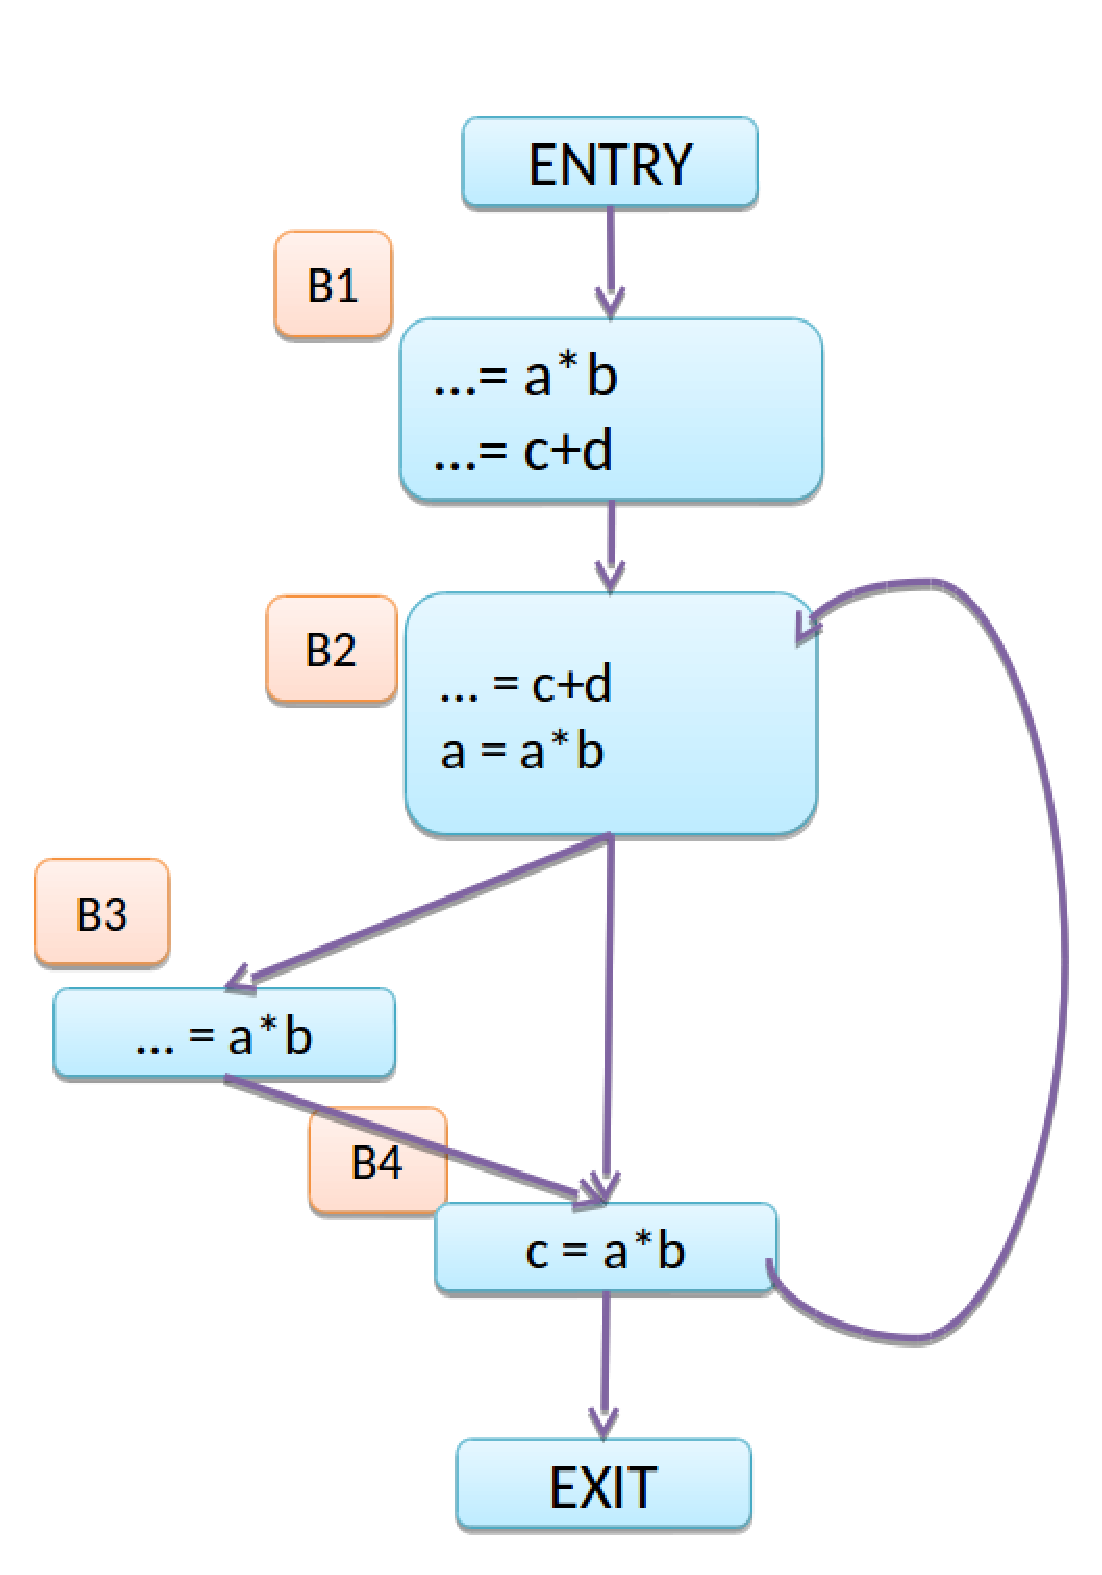
\includegraphics[width=120bp]{AvE_Examp.eps}    
  \end{minipage}\pause
  \begin{minipage}{.45\textwidth}
  \begin{tabular}[t]{|c|c|c|}
    \hline
        {\bf BB} & {\bf \Gen}     & {\bf \Kill} \\ \hline \hline
        B1       & \only<3->{\{a*b, c+d\}} & \only<4->{\{ \}} \\ \hline 
        B2       & \only<5->{\{c+d\}}     & \only<6->{\{a*b\}} \\ \hline 
        B3       & \only<7->{\{a*b\}}         & \only<8->{\{\}} \\ \hline 
        B4       & \only<9->{\{a*b\}}         & \only<10>{\{c+d\}} \\ \hline 
  \end{tabular}\\\bigskip
  \ \\
  \univ = \{a*b, c+d\}
  \end{minipage}
}

\frame{
  \frametitle{Available Expressions: Example}
  \begin{minipage}{.4\textwidth}
  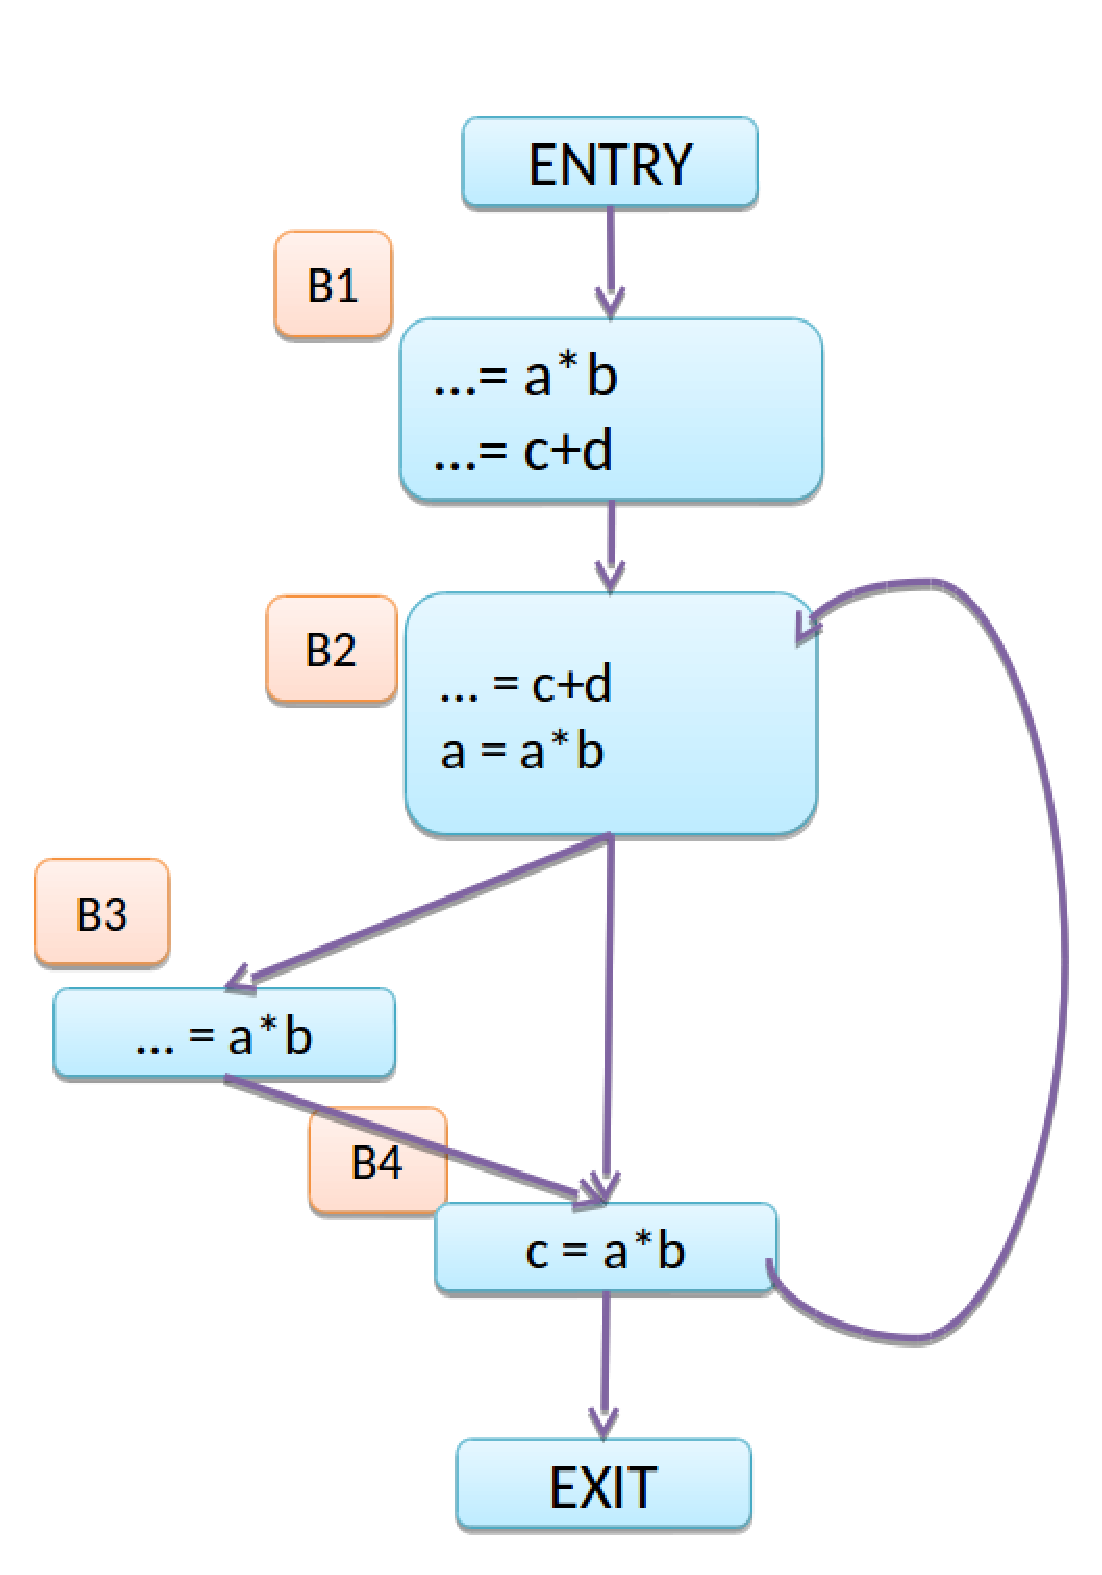
\includegraphics[width=120bp]{AvE_Examp.eps}    
  \end{minipage}
  \begin{minipage}{.45\textwidth}\scriptsize
  \begin{tabular}[t]{|@{}c@{}|@{}c@{\ }||p{8mm}|p{9mm}|p{8mm}|p{8mm}|}
    \hline
        {\bf Pass\#} & {\bf Pt} & {\bf B1} & {\bf B2} & {\bf B3} & {\bf B4}
        \\ \hline \hline
        Init & \IN  & - & - & - & -  \\ \cline{2-6} 
        & \OUT & $\univ$ & $\univ$ & $\univ$ & $\univ$ \\\hline
        \pause
        1 & \IN & $\emptyset$ & a*b, c+d & c+d & c+d \\ \cline{2-6}
        & \OUT & a*b, c+d & c+d& a*b, c+d& a*b \\ \hline
        \pause
        2 & \IN & $\emptyset$ & a*b & c+d & c+d \\ \cline{2-6}
        &\OUT & a*b, c+d& c+d & a*b, c+d & a*b \\ \hline 
        \pause
        3 & \IN & $\emptyset$ & a*b & c+d & c+d \\ \cline{2-6}
        &\OUT & a*b, c+d& c+d & a*b, c+d & a*b \\ \hline 
  \end{tabular}
  \end{minipage}
}

\frame{
  \frametitle{Available Expressions: Bitvectors}
  \begin{minipage}{.4\textwidth}
  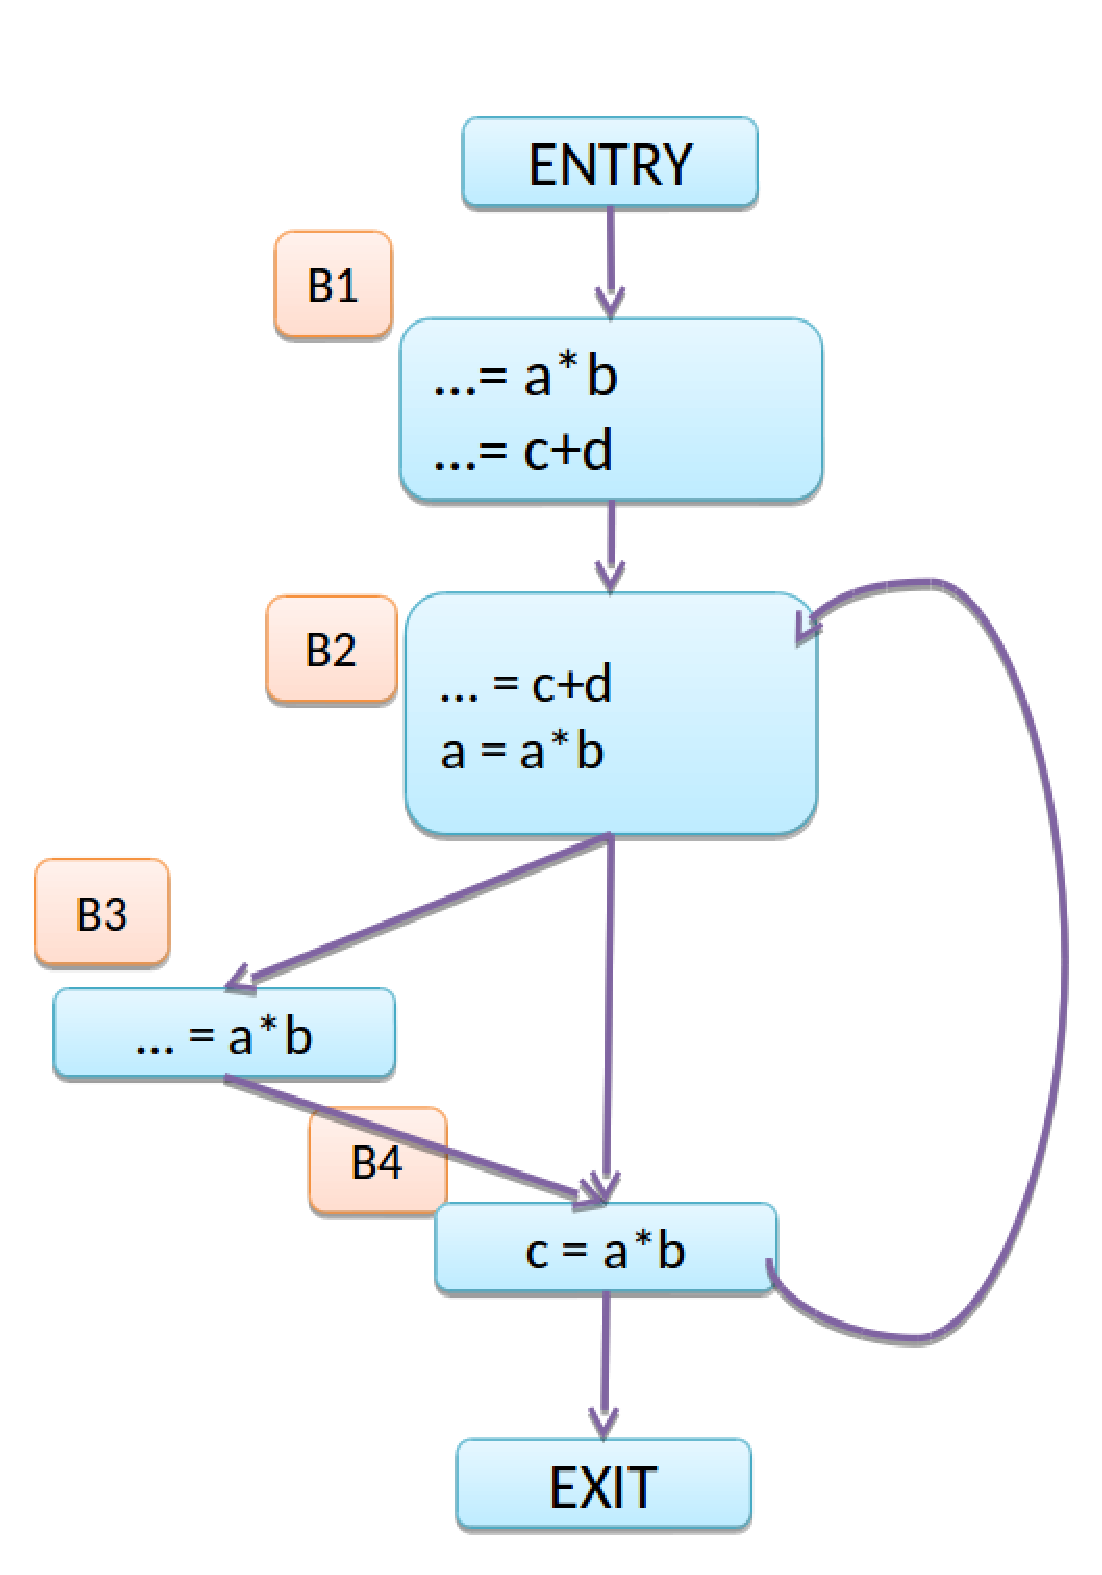
\includegraphics[width=120bp]{AvE_Examp.eps}    
  \end{minipage}
  \begin{minipage}{.45\textwidth}\scriptsize
    a bit for each expression: \\
    \begin{tabular}{|@{\ }c@{\ }|@{\ }c@{\ }|}
      \hline a*b & c+d  \\ \hline
    \end{tabular} \pause
    
  \begin{tabular}[t]{|@{}c@{}|@{}c@{\ }||@{\ }c@{\ }|@{\ }c@{\ }|@{\ }c@{\ }|@{\ }c@{\ }|}
    \hline
        {\bf Pass\#} & {\bf Pt} & {\bf B1} & {\bf B2} & {\bf B3} & {\bf B4}
        \\ \hline \hline
        Init & \IN  & - & - & - & -  \\ \cline{2-6} 
         & \OUT & 11 & 11 & 11 & 11 \\\hline
        1 & \IN & 00 & 11 & 01 & 01 \\ \cline{2-6}
        & \OUT  & 11 & 01 & 11 & 10 \\ \hline
        2 & \IN & 00 & 10 & 01 & 01 \\ \cline{2-6}
        & \OUT  & 11 & 01 & 11 & 10 \\ \hline 
        3 & \IN & 00 & 10 & 01 & 01 \\ \cline{2-6} 
        & \OUT  & 11 & 01 & 11 & 10 \\ \hline 
  \end{tabular}
  \end{minipage}
}

\frame{
  \frametitle{Available Expressions: Bitvectors}
  \begin{itemize}[<+->]
  \item Set-theoretic  definitions:
    \[\IN(B) = \bigcap_{P\in\Pred(B)} \OUT(P)\]
    \[ \OUT(B) = \IN(B) - \Kill(B) \cup \Gen(B) \]
  \item Bitvector definitions:
    \[\IN(B) = \bigwedge_{P\in\Pred(B)} \OUT(P)\]
    \[ \OUT(B) = \IN(B) \wedge \neg\Kill(B) \vee \Gen(B) \]
  \item Bitwise $\vee, \wedge, \neg$ operators
  \end{itemize}
}

\frame{
  \frametitle{Available Expressions: Application}
  \begin{itemize}[<+->]
  \item Common subexpression elimination in a block $B$
    \begin{itemize}
    \item Expression $e$ available at the entry of $B$
    \item $e$ is also computed at a point $p$ in $B$
    \item Components of $e$ are not modified from entry of $B$ to $p$
    \end{itemize}
  \item $e$ is ``upward exposed'' in $B$
  \item Expressions generated in $B$ are ``downward exposed''
  \end{itemize}
}

\frame{
  \frametitle{Comparison of RD and AvE}
  \begin{itemize}[<+->]
  \item {\em Some} vs. {\em All} path property
  \item Meet operator: $\cup$ vs. $\cap$
  \item Initialization of \bbent: $\emptyset$ 
  \item Initialization of other BBs: $\emptyset$ vs. $\univ$
  \item Safety: ``More'' RD vs. ``Fewer'' AvE
  \end{itemize}
}

\frame{
  \frametitle{AvE: alternate Initialization}
  \begin{itemize}[<+->]
  \item What if we Initialize:
    \[ \OUT(B) = \emptyset, \forall B \mbox{ including \bbent} \]
  \item Would we find ``extra'' available expressions?
    \begin{itemize}
    \item More opportunity to optimize?
    \end{itemize}
  \item OR would we miss some expressions that are available?
    \begin{itemize}
    \item Loose on opportunity to optimize?
    \end{itemize}
  \end{itemize}
}

\frame{
  \frametitle{Live Variables}
  \begin{itemize}[<+->]
  \item A variable $x$ is live at a point $p$ if
    \begin{itemize}
    \item There is a point $p'$ along some path in the flow graph
      starting at $p$ to the \bbext
    \item Value of $x$ could be used at $p'$
    \item There is no definition of $x$ between $p$ and $p'$
      along this path
    \end{itemize}
  \item Otherwise $x$ is dead at $p$
  \end{itemize}
}

\frame{
  \frametitle{Live Variables: \Gen}
  \begin{itemize}
  \item $\Gen(B)$: Set of variables whose values may be used in
    block $B$ prior to any definition
    \begin{itemize}
    \item Also called ``use($B$)''
    \end{itemize}
  \item ``upward exposed use'' of a variable in $B$
  \end{itemize}
}

\frame{
  \frametitle{Live Variables: \Kill}
  \begin{itemize}
  \item $\Kill(B)$: Set of variables defined in 
    block $B$ prior to any use
    \begin{itemize}
    \item Also called ``def($B$)''
    \end{itemize}
  \item ``upward exposed definition'' of a variable in $B$
  \end{itemize}
}
\frame{
  \frametitle{Live Variables: Equations}
  \begin{itemize}[<+->]
  \item Set-theoretic  definitions:
    \[ \OUT(B) = \bigcup_{S\in\Succ(B)} \IN(S)\]
    \[ \IN(B) = \OUT(B) - \Kill(B) \cup \Gen(B) \]
  \item Bitvector definitions:
    \[ \OUT(B) = \bigvee_{S\in\Succ(B)} \OUT(S)\]
    \[ \IN(B) = \OUT(B) \wedge \neg\Kill(B) \vee \Gen(B) \]
  \item Bitwise $\vee, \wedge, \neg$ operators
  \end{itemize}
}

\frame{
  \frametitle{Very Busy Expressions}
  \begin{itemize}[<+->]
  \item Expression $e$ is very busy at a point $p$ if
    \begin{itemize}
    \item {\em Every} path from $p$ to \bbext has at least one
      evaluation of $e$
    \item On every path, there is no assignment to any component
      variable of $e$ before the first evaluation of $e$ following
      $p$
    \end{itemize}
  \item Also called {\em Anticipable expression}
  \end{itemize}
}

\frame{
  \frametitle{QQ}
  \begin{itemize}
  \item Expression $e$ is very busy at a point $p$ if
    \begin{itemize}
    \item {\bf Every} path from $p$ to \bbext has at least one
      evaluation of $e$ and there is no assignment to any component
      variable of $e$ before the first evaluation of $e$ following
      $p$ on these paths.
    \end{itemize}
  \item Set up the data flow equations for Very Busy Expressions
    (VBE). You have to give equations for \Gen, \Kill, \IN, and
    \OUT.
  \item Think of an optimization/transformation that uses VBE
    analysis. Briefly describe it (2-3 lines only)
  \item Will your optimization be {\em safe} if we replace ``{\em
    Every}'' by ``{\em Some}'' in the definition of VBE?
  \end{itemize}
}
\end{document}

